\subsubsection{Memory Model}

While at the device level, synchronization is allowed via device-specific mechanics, that is not the case at the host level. When considering the whole host, or the entire group of available devices, a problem arises as each device possesses its own private memory address space, creating an obstacle to efficiently take advantage of the computational resources. Thus, a Global Memory System (GMS) is employed, using a relaxed consistency model requiring explicit memory ences to ensure full data consistency. 

\begin{figure}[!htp]
  \centering
  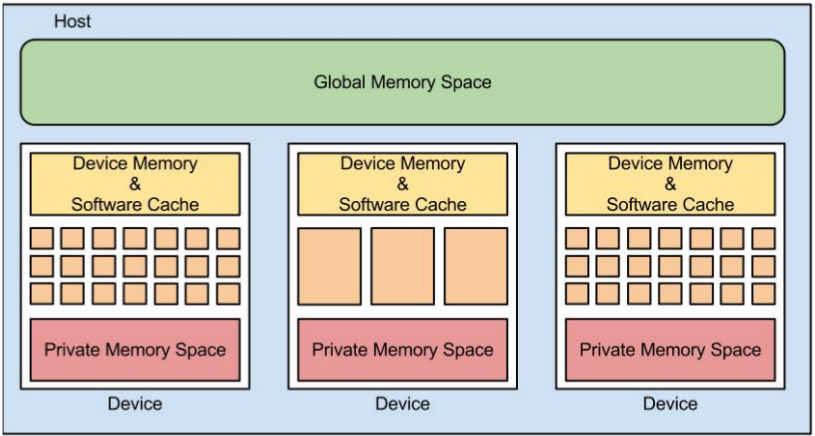
\includegraphics[width=0.6\columnwidth]{UPEM.png}
  \caption{GAMA Memory and Execution Model}
  \label{fig:upem}
\end{figure}

\Cref{fig:upem} provides an overview of the memory model employed in GAMA. It is based on a hierarchy, composed of three levels:
\begin{itemize}
  \item The first level is private and refers to a memory space addressable only by a single task
  \item The second level is shared between all Computational Units of a single device, and thus can be shared accross tasks that are running on the same device. It is not addressable by other devices, however.
  \item Finally, the global level is addressable by the entire host system. However, due to implementation details of atomic operations being undefined, this level uses a relaxed consistency model, and requires explicit synchronization barriers to be used in order to ensure data consistency. 
\end{itemize}

Besides the memory hierarchy, GAMA also employs a software cache to reduce latency in global memory space accesses and to exploit potential temporal and spatial locality. This cache is tipycally implemented over the private memory address space of each device, and can also operate as a pre-fetch mechanism, as it has the ability of copying memory blocks to the device in which they are required, prior to the execution of the corresponding task.
